\subsection{Detailed schematic of the open loop system}
The detailed schematic of the open loop studied system is shown in figure \ref{fig:detailed_schematic}.
\begin{figure}[H]
    \centering
    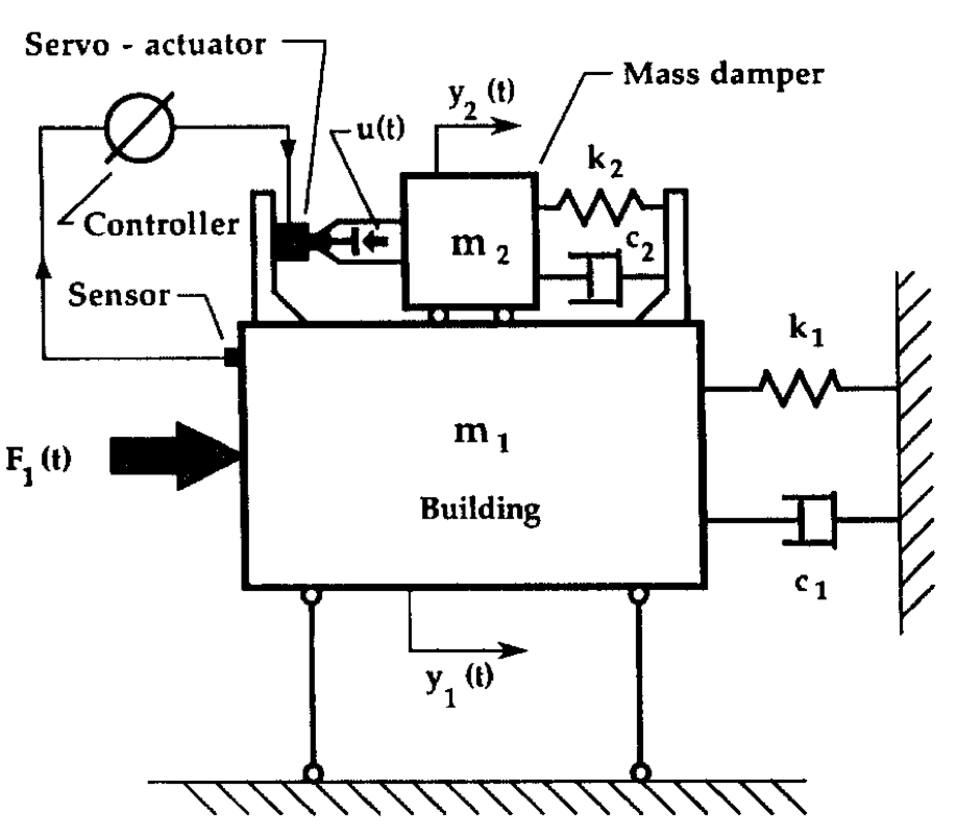
\includegraphics[width=0.7\textwidth]{resources/pdf/schema.pdf}
    \caption{Detailed schematic of the open loop studied system \cite{science_direct}}
    \label{fig:detailed_schematic}
\end{figure}
The building is represented by the mass $m_1$ and its oscillation motion is simulated by the spring $k_1$ and the damper $c_1$.\par
The mass damper is represented by the mass $m_2$ and its movement is simulated by the spring $k_2$ and the damper $c_2$.\par
The force $F_1(t)$ represents the wind force (uncontrollable) on the building.\par
The force $u(t)$ represents the force applied on the mass damper by the controller (controllable).\par
We are studying, at first, our system without a control mechanism. Our controllable input $u(t)$ will therefore be \num{0} for all our simulations in this section.
